% Created 2024-08-04 Sun 17:41
% Intended LaTeX compiler: lualatex
\documentclass[presentation,professionalfonts,smaller,aspectratio=169]{beamer}
                

% 
\makeatletter
 \@ifclassloaded{beamer}{%
  %%% save beamer's `solution' environment as `beamersolution':
  \let\beamersolution\solution
  \let\endbeamersolution\endsolution
  %%% "delete" the `solution' environment:
  \let\solution\relax
  \let\endsolution\relax
}{%
}%
\makeatother
\usepackage[utf8]{inputenc}
\usepackage[T1]{fontenc}
%\usepackage[french]{babel}
\usepackage[portuguese]{babel}

%%%% FONTS




\usepackage{xsim}
\usepackage[most]{tcolorbox}
\usepackage{amssymb}
\usepackage{fontawesome}
\newcounter{paragraph}



\DeclareExerciseEnvironmentTemplate{custom}{%
  \begin{tcolorbox}[boxrule = 0pt]
  \tcbox[on line,colback=teal,colframe=teal,coltext=white,size=small]{%
    \faBook\sffamily\bfseries\
    \XSIMmixedcase{\GetExerciseName}
    \GetExerciseProperty{counter}%
  }\quad
}{\end{tcolorbox}}


\DeclareExerciseEnvironmentTemplate{custom2}{%
  \begin{tcolorbox}[boxrule = 0pt]
  \tcbox[on line,colback=violet,colframe=violet,coltext=white,size=small]{%
    \faToggleOn\sffamily\bfseries\
    \XSIMmixedcase{\GetExerciseName}
    \GetExerciseProperty{counter}%
  }\quad
}{\end{tcolorbox}}




\DeclareExerciseType{test}{
	exercise-env = question ,
	solution-env = answer ,
	exercise-template = custom ,
	solution-template = custom2 ,
	exercise-name	= Exemplo. ,
	exercises-name = Exemplo ,
	solution-name = Solução ,
	solutions-name = Sol. ,
	exercise-heading = \textbf ,
	solution-heading = \textbf
}


\xsimsetup{
  exercise/within = section,
  exercise/the-counter =  \arabic{exercise}, 
%%solution-name = solution,  % used with headings=true
solution/print=false,
%print-collection/print=both,
}





\usepackage{colortbl}
\usepackage[tikz]{bclogo}
\usetikzlibrary{fit,patterns,shadows.blur,shapes,mindmap}
\usetikzlibrary{arrows,calc,arrows.meta,decorations.markings,shapes.symbols}
\usetikzlibrary{decorations.pathreplacing, decorations.pathmorphing,calc,arrows,positioning}
\usepackage{tikzpeople}
\usepackage{qrcode,hyperref}
\usepackage{upgreek}
%\usepackage[version=4]{mhchem}
\usepackage{tabularray}


\NewTblrTheme{fancy}{
\SetTblrStyle{caption-tag}{font=\bfseries}
\SetTblrInner[tblr,longtblr]{rowsep=2.5pt}
\DefTblrTemplate{firsthead, middlehead,lasthead}{default}{} % <---
\DefTblrTemplate{contfoot-text}{normal}{\scriptsize\textit{Continued on the next page}}
\SetTblrTemplate{contfoot-text}{normal}
}






\usepackage{chemfig,chemmacros,elements,chemformula}
\chemsetup{modules={all}}
\chemsetup[redox]{pos=top,roman=false}
\chemsetup[redox]{pos=top}
\chemsetup{redox/sep=.5em}
\chemsetup[redox]{explicit-sign=true}
\NewChemPhase\lqdd{\(\ell\)}
\NewChemPhase\gr{grafite}
\NewChemPhase\reac{reação}
\NewChemState\Enthalpy{symbol=H,superscript=,unit=\kilo\joule}%
\usepackage{siunitx}
\setchemfig{fixed length=false, atom sep=2.5em, arrow offset=6pt, scheme debug=false}%,angle increment=30}
\renewcommand*\printatom[1]{\ensuremath{\mathsf{#1}}} % This line changes the font of the atoms to sans serif
%%%% QRCODE
\usepackage{pdfpages}
\usepackage{mol2chemfig}
\usepackage{subfig,caption}
\usepackage{wrapfig}
\usepackage{enumitem}
\setitemize{label=\usebeamerfont*{itemize item}%
\usebeamercolor[fg]{itemize item}
\usebeamertemplate {itemize item}}
\usepackage{array} % ajust colunm table
\usepackage{cancel}
\usepackage[controls]{animate}
\renewcommand{\CancelColor}{\color{red}}

%%%%%%%%%%%%%%%%%%% CONFIG TCOLORBOX 

\newtcolorbox{mybox}[2][]{boxsep=0.5em,left=0.5em,
colback=blue!5!white, colframe=blue!75!black,
fonttitle=\bfseries\sffamily,
colbacktitle=blue!85!red!60,enhanced,
attach boxed title to top left={yshift=-3mm,xshift=5mm},
title=#2,#1}

\newtcolorbox{myrule}[2][]{boxsep=0.5em,left=0.5em,
colback=green!5!white, colframe=blue!75!black,
fonttitle=\bfseries\sffamily,
colbacktitle=blue!85!red!60,enhanced,
attach boxed title to top left={yshift=-3mm,xshift=5mm},
title=#2,#1}


\newtcolorbox{myex}[2][]{boxsep=0.5em,left=0.5em,
  colback=yellow!5!white, colframe=blue!75!black, 
  fonttitle=\bfseries\sffamily,
  colbacktitle=blue!85!red!60,enhanced,
  attach boxed title to top left={yshift=-3mm,xshift=5mm},
  title=#2,#1}


 \definecolor{col1}{HTML}{FF7878}
 \definecolor{col2}{HTML}{51B5F8}
 \definecolor{col3}{HTML}{68E1AA}
 \definecolor{col4}{HTML}{B869EA}
 \definecolor{col5}{HTML}{FF5500}
 \definecolor{col6}{HTML}{FFF8E7}
 \definecolor{col7}{HTML}{FF9966}
 \definecolor{col8}{HTML}{9400D3}



\definesubmol\nobond{-[,0.2,,,draw=none]\scriptstyle\color{blue}}
\newcommand{\re}{\hspace{-1cm}}
\newcommand{\af}{\hspace{2cm}}

%%%% Config X sim for BEAMER
\makeatletter
\@ifclassloaded{beamer}{%
%%% save beamer's `solution' environment as `beamersolution':
\let\beamersolution\solution
\let\endbeamersolution\endsolution
%%% "delete" the `solution' environment:
\let\solution\relax
\let\endsolution\relax
}{%
}%
\makeatother
\usepackage[utf8]{inputenc}
\usepackage[T1]{fontenc}
%\usepackage[portuguese, ]{babel}
%%%% FONTS
%%% XSIM CONFIG BEAMER
\usepackage{xsim}
\usepackage[most]{tcolorbox}
\usepackage{amssymb}
\usepackage{fontawesome}
\usepackage{tasks}
\newcounter{paragraph}
\usepackage[dvipsnames,svgnames]{xcolor}
\usepackage{annotate-equations}
%%% BOX EXERCISE BEAMER
\DeclareExerciseEnvironmentTemplate{custom}{%
\begin{tcolorbox}[boxrule = 0pt]
\tcbox[on line,colback=teal,colframe=teal,coltext=white,size=small]{%
\faBook\sffamily\bfseries\
\XSIMmixedcase{\GetExerciseName}
\GetExerciseProperty{counter}%
}\quad
}{\end{tcolorbox}}
%% == CUSTOM BOX BEAMER
\DeclareExerciseEnvironmentTemplate{custom2}{%
\begin{tcolorbox}[boxrule = 0pt]
\tcbox[on line,colback=violet,colframe=violet,coltext=white,size=small]{%
\faToggleOn\sffamily\bfseries\
\XSIMmixedcase{\GetExerciseName}
\GetExerciseProperty{counter}%
}\quad
}{\end{tcolorbox}}
\DeclareExerciseType{test}{
exercise-env = question ,
solution-env = answer ,
exercise-template = custom ,
solution-template = custom2 ,
exercise-name = Exemplo. ,
exercises-name = Exemplo ,
solution-name = Solução ,
solutions-name = Sol. ,
exercise-heading = \textbf ,
solution-heading = \textbf
}
\xsimsetup{
exercise/within = section,
exercise/the-counter =  \arabic{exercise},
%%solution-name = solution,  % used with headings=true
solution/print=false,
print-collection/print=both,
}
\NewTasksEnvironment[label = (\emph{\alph*}),
label-width = 12pt]{choice}[\choice]
\usepackage{colortbl}
\usepackage[tikz]{bclogo}
\usetikzlibrary{fit,patterns,shadows.blur,shapes,mindmap}
\usetikzlibrary{arrows,arrows.meta,decorations.markings,shapes.symbols}
\usetikzlibrary{decorations.pathreplacing, decorations.pathmorphing,calc,arrows,positioning}
\usepackage{tikzpeople}
\usepackage{qrcode,hyperref}
\usepackage{upgreek}
%\usepackage[version=4]{mhchem}
\usepackage{tabularray}
%%% CUSTOM TABLE
\NewTblrTheme{fancy}{
\SetTblrStyle{caption-tag}{font=\bfseries,red2}
\SetTblrInner[tblr,longtblr]{rowsep=2.5pt}
\DefTblrTemplate{firsthead, middlehead,lasthead}{default}{} % <---
\DefTblrTemplate{contfoot-text}{normal}{\scriptsize\textit{Continua ...}}
\SetTblrTemplate{contfoot-text}{normal}
}
%% ==== CHEMMACROS E CHEMFIG CONFIG
\usepackage{chemfig,chemmacros,elements,chemformula}
\chemsetup{modules={all}}
\chemsetup[redox]{pos=top,roman=false}
\chemsetup[redox]{pos=top}
\chemsetup{redox/sep=.5em}
\chemsetup[redox]{explicit-sign=true} %%% reaction redox
%% == CUSTOM PHASES IN CHEMMACROS
\NewChemPhase\lqdd{\(\ell\)}
\NewChemPhase\gr{grafite}
\NewChemPhase\reac{reação}
\NewChemState\Enthalpy{symbol=H,superscript=,unit=\kilo\joule}%
\usepackage{siunitx}
\setchemfig{fixed length=false, atom sep=2.5em, arrow offset=6pt, scheme debug=false}
%% == NUMEROS PARA FORMULES
\renewcommand*\printatom[1]{\ensuremath{\mathsf{#1}}} % This line changes the font of the atoms to sans serif
%%% INCLUDE PAGES PDFs
\usepackage{pdfpages}
\usepackage{mol2chemfig}
\usepackage{subfig,caption}
\usepackage{wrapfig}
\usepackage{enumitem}
\setitemize{label=\usebeamerfont*{itemize item}%
\usebeamercolor[fg]{itemize item}
\usebeamertemplate {itemize item}}
\usepackage{array} % ajust colunm table
\usepackage{cancel}
\usepackage[controls]{animate}
\renewcommand{\CancelColor}{\color{red}}
%%%%%%%%%%%%%%%%%%% CONFIG TCOLORBOX
\newtcolorbox{mybox}[2][]{boxsep=0.5em,left=0.5em,
colback=blue!5!white, colframe=blue!75!black,
fonttitle=\bfseries\sffamily,
colbacktitle=blue!85!red!60,enhanced,
attach boxed title to top left={yshift=-3mm,xshift=5mm},
title=#2,#1}
\newtcolorbox{myrule}[2][]{boxsep=0.5em,left=0.5em,
colback=green!5!white, colframe=blue!75!black,
fonttitle=\bfseries\sffamily,
colbacktitle=blue!85!red!60,enhanced,
attach boxed title to top left={yshift=-3mm,xshift=5mm},
title=#2,#1}
\newtcolorbox{myex}[2][]{boxsep=0.5em,left=0.5em,
colback=yellow!5!white, colframe=blue!75!black,
fonttitle=\bfseries\sffamily,
colbacktitle=blue!85!red!60,enhanced,
attach boxed title to top left={yshift=-3mm,xshift=5mm},
title=#2,#1}
\definecolor{col1}{HTML}{FF7878}
\definecolor{col2}{HTML}{51B5F8}
\definecolor{col3}{HTML}{68E1AA}
\definecolor{col4}{HTML}{B869EA}
\definecolor{col5}{HTML}{FF5500}
\definecolor{col6}{HTML}{FFF8E7}
\definecolor{col7}{HTML}{FF9966}
\definecolor{col8}{HTML}{9400D3}
%% CONFIG COLOR CARBONO
\tikzstyle{bal}=[inner sep=0.3pt,fill=orange,fill opacity=0.5,circle,minimum size=0.2cm]
\tikzstyle{rect}=[inner sep=0.3pt,fill=red,fill opacity=0.5,circle,minimum size=0.2cm]
\tikzstyle{bal2}=[inner sep=0.3pt,fill=blue,fill opacity=0.5,circle,minimum size=0.2cm]
\tikzstyle{bal3}=[inner sep=0.3pt,fill=yellow,fill opacity=0.5,circle,minimum size=0.2cm]
\definesubmol\nobond{-[,0.2,,,draw=none]\scriptstyle\color{blue}}
\newcommand{\re}{\hspace{-1cm}}
\newcommand{\af}{\hspace{2cm}}
\date{}
%\usetheme{minflat}
\DeclareExerciseCollection{Hidro}
\usetheme{minflat}
\author{Fábio Lima}
\date{}
\title{Hidrocarbonetos}
\hypersetup{
 pdfauthor={Fábio Lima},
 pdftitle={Hidrocarbonetos},
 pdfkeywords={},
 pdfsubject={},
 pdfcreator={Emacs 29.4 (Org mode 9.6.15)}, 
 pdflang={En Portuguese}}
\begin{document}

\maketitle
\begin{frame}{Sumário}
\tableofcontents
\end{frame}




\section{Introdução}
\label{sec:org3ab3dc5}

\begin{frame}[label={sec:org93852bd}]{Breve Histórico}
\begin{mybox}{Precusores}


\begin{itemize}
\item 1807 - Jöns J. Berzelius – Teoria da Força Vital.
\item 1828 – primeiro composto orgânico sintetizado em laboratório – Uréia
\end{itemize}
\begin{center}
\schemestart
\chemname{\chemfig{NH_4CNO}}{Cianato \\ de amônio}
\arrow{->[\(\Delta\)][]}
\chemname{\chemfig{O=C([:30]-NH_2)([:330]-NH_2)}}{Ureia}
\schemestop
\end{center}

\begin{itemize}
\item Tudo que tem “vida” possui compostos orgânicos,mas nem todos compostos orgânicos possuem vida.
\item 1851 à 1861 – Friederich A. Kekulé
\begin{itemize}
\item Formulou três postulados que vigoram até hoje.
\end{itemize}
\end{itemize}
\end{mybox}
\end{frame}


\begin{frame}[label={sec:org3446d40}]{Postulados de Kekulé}
\begin{myrule}{Postulado 1}

\begin{itemize}
\item Os átomos de carbono são tetravalentes.
\end{itemize}
\begin{center}
\chemfig{H-C([:90]-H)([:-90]-H)-C([:90]-H)([:-90]-H)-H}
\end{center}

\begin{itemize}
\item Ligações Covalentes
\end{itemize}

\begin{center}
\chemfig{H-C~C-C([:90]-H)([:-90]-H)-H}
\end{center}

\end{myrule}
\end{frame}


\begin{frame}[label={sec:orgc4f55f0}]{Ligações Múltiplas}

\begin{talltblr}[
	 theme= fancy,
	 caption={Composição do Petróleo},
	 ]{
	 colspec = {Xcc}, colsep = 2mm, hlines = {2pt, white},
	 %row{odd} = {brown8}, row{even} = {gray8},
	 row{1} = {2em,azure2,fg=white,font=\bfseries\sffamily},
	 }
	 \hline
	 Tipo de Ligação & Exemplo & Estrutura de Lewis\\[0pt]
	 \hline
	 Ligação \alert{dupla} entre dois átomos de carbono & \chemfig{C([:210]-)([:150]-)=C([:30]-)([:330]-)} & \chlewis{0:120.240.}{C}  \chlewis{180:60.290.}{C}\\
	 \hline
	 Ligação \alert{dupla} entre um átomo de oxigênio e carbono & \chemfig{C([:210]-)([:150]-)=O} & \chlewis{0:120.240.}{C} \chlewis{180:90:0:}{O}\\
	 \hline
	  Ligação \alert{tripla} entre dois átomos de carbono & \chemfig{-C~C-} & \chlewis{0:50.180.}{C} \chlewis{180:130.0.}{C}\\
	 \hline
	 Ligação \alert{tripla} entre um carbono e nitrogênio & \chemfig{-C~N } & \chlewis{0:50.180.}{C} \chlewis{180:130.0:}{N}\\[0pt]
	 \hline
 \end{talltblr}
\end{frame}


\begin{frame}[label={sec:org0492536}]{Postulados de Kekulé}
\begin{myrule}{Postulado 2}


\begin{itemize}
\item As quatro valências do carbono são equivalentes.
\end{itemize}

\begin{figure}[htbp]
\centering
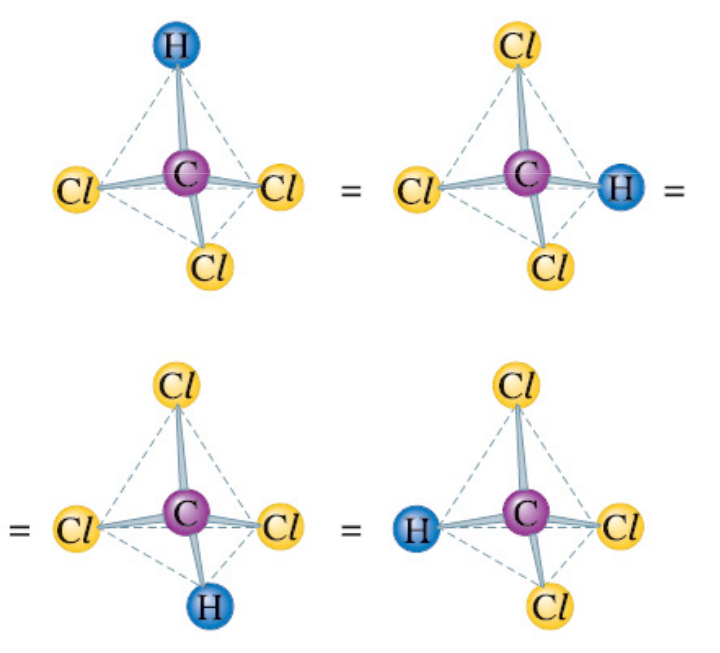
\includegraphics[width=0.45\textwidth]{QO/Fundamentos/cloroformio.png}
\caption{\label{fig:org3d0a65c}Clorofórmio}
\end{figure}

\end{myrule}
\end{frame}


\begin{frame}[label={sec:org5a39d70}]{Postulados de Kekulé}
\begin{myrule}{3º Postulado}

\begin{itemize}
\item O carbono possui a capacidade \alert{ÚNICA} de formas cadeias.
\end{itemize}



\begin{tblr}{cc}
\chemfig{H-C([:90]-H)([:-90]-H)-C([:-90]-H)=C([:-90]-H)-C([:90]-H)([:-90]-H)-H}& 
\chemfig{C*6((-H)=C(-H)-C(-H)=C(-H)-C(-H)=C(-H)-)} \\
\chemfig{H-[:210]C(-[:120]H)-[:300]C(-[:20]C(-[:320]H)(-[:20]H)-[:80]H)(-[:300]H)-[:210]C(-[:300]H)(-[:210]H)-[:120]C(-[:30]\phantom{C})(-[:210]H)-[:120]H} & 
%\qquad \qquad \chemfig{>[:330](-[:330]-[:30]-[:330])(<:[:60])-[:210](-[:270])-[:150](-[:90])-[:210]-[:150]}
\chemfig{H-[:276]C(-[:12]H)-[:180]C(-[:84]H)(-[:168]H)-[:252]C(-[:156]H)(-[:240]H)-[:324]C(-[:228]H)(-[:312]H)-[:36]C(-[:108]\phantom{C})(-[:24]H)-[:300]H}\\
\end{tblr}

\end{myrule}
\end{frame}


\section{Carbonos}
\label{sec:orgcf90f7e}

\begin{frame}[label={sec:org3ee99aa}]{Classificação dos carbonos}
\begin{center}
\begin{tabular}{|c|c|}
\hline
\cellcolor{green!20} {\bfseries Carbono}  & \cellcolor{green!20} {\bfseries Definição} \\[0pt]
\hline
Primário & ligado diretamente, \alert{no máximo}, a \alert{1} outro carbono\\[0pt]
\hline
Secundário & ligado diretamente a \alert{2} outros carbonos\\[0pt]
\hline
Terciário & ligado diretamente  a \alert{3} outros carbonos\\[0pt]
\hline
Quartenário & ligado diretamente a \alert{4} outros carbonos\\[0pt]
\hline
\end{tabular}
\end{center}



\begin{columns}
\begin{column}{0.7\textwidth}
\chemfig[scale=2.5]{H_3@{A}C-@{L}C([:-90]-@{B}CH_3)=@{F}CH-@{G}C~@{H}C-@{N}C([:90]-@{D}CH_3)([:-90]-@{K}CH_2(-[:270,,1,1]@{M}CH-[:300,,1,1]@{J}CH_2-[:180,,1,2]H_2@{I}C(-[:60,,2]\phantom{C})))-@{E}CH_3}
\chemmove{
\node[bal,fit=(A)]{};
\node[bal,fit=(B)]{};
\node[bal,fit=(D)]{};
\node[bal,fit=(E)]{};
\node[rect,fit=(F)]{};
\node[rect,fit=(G)]{};
\node[rect,fit=(H)]{};
\node[rect,fit=(I)]{};
\node[rect,fit=(J)]{};
\node[rect,fit=(K)]{};
\node[bal2,fit=(L)]{};
\node[bal2,fit=(M)]{};
\node[bal3,fit=(N)]{};
}
\end{column}
\begin{column}{0.3\textwidth}  %%<--- here
      carbonos \chemfig{@{A}C} = primários\\
      carbonos \chemfig{@{B}C} = secundários\\
      carbonos \chemfig{@{D}C} = terciários\\
      carbonos \chemfig{@{E}C} = quartenários
     \chemmove{
      \node[bal,fit=(A)]{};
      \node[rect,fit=(B)]{};
      \node[bal2,fit=(D)]{};
      \node[bal3,fit=(E)]{};
      }
\end{column}
\end{columns}
\end{frame}


\section{Cadeias}
\label{sec:org056cea9}

\begin{frame}[label={sec:org3426f02}]{Cadeias Carbônicas}
\begin{myrule}{Heteroátomo}

\begin{itemize}
\item Estrutura formada por todos os átomos de carbono e os heteroátomos.
\item Heteroátomo é um átomo diferente do carbono e do hidrogênio  posicionado
entre  dois  carbonos  na cadeia.
\end{itemize}

\chemname{\chemfig{CH_3-CH_2-{\color{red}O}-CH_2-CH_3}}{Oxigênio é heteroátomo}

\vspace{.5cm}\chemname{\chemfig{CH_3-CH_2-CH_2-CH_2-{\color{red}O}H}}{Oxigênio NÃO é heteroátomo}

\end{myrule}
\end{frame}




\begin{frame}[allowframebreaks]{Classificação das Cadeias Carbônicas}
\begin{myrule}{Cadeia aberta}

\begin{itemize}
\item \emph{Cadeia aberta ou aciclíca:} Os átomos de carbono se ligam entre si de modo a terem os extremos livres
\end{itemize}

\begin{center}
\schemestart
\chemfig{-@{b}{C}([:90]-)([:-90]-)-C([:90]-)([:-90]-)-C([:90]-)([:-90]-)-@{a}{C}([:90]-)([:-90]-)-}
\schemestop 
\chemmove{\draw[<-,red,shorten <=3.5pt] (b) (-0.5,-0.2)--++(1,-0.4) node[below] {extremo livre} ;
\draw[->,red,shorten <=3.5pt] (a) (-4.7,-.9)--++(1.5,0.7) node[anchor=35,inner sep=23] {extremo livre} ;
}
\vspace{1cm}
%
\end{center}

\end{myrule}


\begin{myrule}{Cadeia Fechada}

\begin{itemize}
\item \emph{Cadeia fechada ou ciclíca:} Os átomos de carbono se ligam entre si de modo a formarem um ciclo.
\end{itemize}

\begin{center}
\chemfig{-[:90]C(-[:180])-C(-[:270])(-)-[:90]C(-)(-[:90])-[:180]C(-[:270]\phantom{C})(-[:90])-[:180]}
\end{center}

\end{myrule}


\begin{myrule}{Cadeia Mista}

\begin{itemize}
\item Os atomos se ligam formando um ciclo e tem as extremidades livres.
\end{itemize}
\begin{center}
\chemfig{-[:90]C(-[:180])-C(-[:90]C(-)(-[:90])-[:180]C(-[:90])(-[:180])-[:270]\phantom{C})(-[:270])-C(-[:270])(-[:90,,,1])-C(-[:90])(-[:270])-C(-[:90])(-)-[:270]}
\end{center}

\end{myrule}
\end{frame}


\section{Cadeias Abertas}
\label{sec:org9c0e8bd}

\begin{frame}[allowframebreaks]{Cadeias Abertas}
\begin{tblr}[
		theme= fancy,
		caption={Classificação das Cadeias},
		]{
			colspec = {XX}, colsep = 2mm, hlines = {2pt, white},
			%row{odd} = {brown8}, row{even} = {gray8},
			row{1} = {2em,azure2,fg=white,font=\bfseries\sffamily},
		}

	Cadeia aberta Normal   &  Cadeia Aberta Ramificada \\
%
		Carbonos, primários, secundários & Ao menos um carbono terciário ou quartenário\\
	\chemfig{-(!\nobond\chemabove[1ex]{}{\color{blue}1})C([:-90]-)([:90]-)-(!\nobond\chemabove[1ex]{}{\color{blue}2})C([:-90]-)([:90]-)-C(!\nobond\chemabove[1ex]{}{\color{blue}3})([:90]-)([:-90]-)-} &  \chemfig{-(!\nobond\chemabove[1ex]{}{\color{blue}1})C([:-90]-)([:90]-)-(!\nobond\chemabove[1ex]{}{\color{blue}2})C([:-90]-C(!\nobond\chemabove[1ex]{}{\color{blue}\hspace{.2cm}\vspace{.7cm}4})([:0]-)([:180]-)-)([:90]-)-C(!\nobond\chemabove[1ex]{}{\color{blue}3})([:90]-)([:-90]-)-}\\
		Carbono 1: primário & \\
		Carbono 2: secundário & Carbono 2: terciário\\
		Carbono 3: primário & Carbonos 1, 3 e 4: primários\\
		\hline
	\end{tblr}




\begin{tblr}[
		theme= fancy,
		caption={Classificação das Cadeias},
		]{
			colspec = {cc}, colsep = 2mm, hlines = {2pt, white},
			%row{odd} = {brown8}, row{even} = {gray8},
			row{1} = {2em,azure2,fg=white,font=\bfseries\sffamily},
		}
  Cadeia aberta homogênea   &  Cadeia aberta heterogênea \\
Apresentam somentes átomos de carbono & Ao menos um átomo heteroátomos\\
 \chemfig{-C([:-90]-)([:90]-)-C([:90]-)=C([:90]-)([:-90]-)-} &  \chemfig{-C([:90]-)([:-90]-)-C([:90]-)([:-90]-)-{\color{blue}O}-C([:90]-)([:-90]-)-} \\
 \chemfig{-C([:90]-)([:-90]-)-C([:90]-)([:-90]-C([:180]-)([:0]-)-)-C([:90]-)([:-90]-)-{\color{red} O}-}  &  \chemfig{-C([:90]-)([:-90]-)-C([:-90]-C([:180]-)([:0]-)-)={\color{blue}N}-C([:90]-)([:-90]-)-C([:90]-)([:-90]-)-} \\
Este \emph{oxigênio} não é heteroátomo & \\
\hline
\end{tblr}



\begin{tblr}[
		theme= fancy,
		caption={Classificação das Cadeias},
		]{
			colspec = {XX}, colsep = 2mm, hlines = {2pt, white},
			%row{odd} = {brown8}, row{even} = {gray8},
			row{1} = {2em,azure2,fg=white,font=\bfseries\sffamily},
		}
Cadeia aberta saturada   &  Cadeia aberta insaturada \\
Apresentam somentes átomos de carbono apresentam ligações simples & Apresenta ao menos dois átomos de  carbono ligados pela dupla ou tripla ligação\\
 \chemfig{-C([:-90]-)([:90]-)-C([:90]-)([:-90]-)-C([:90]-)([:-90]-)-} &  \chemfig{-C([:90]-)([:-90]-)-{\color{blue}C}([:-90]-)={\color{blue}C}([:-90]-)-} \\
 \chemfig{-C([:90]-)([:-90]-)-C([:90]-)([:-90]-C([:180]-)([:0]-)-)-C([:90]-)([:-90]-)-{\color{red} O}-}  &  \chemfig{-C([:90]-)([:-90]-)-C-{\color{blue}C}(~[4,,,,blue]{\color{blue}C})-C([:90]-)([:-90]-)-C([:90]-)([:-90]-)-} \\
O átomo de carbono que apresenta ligação simples é chamado de \emph{carbono saturado}. & A átomo que apresenta ligação dupla ou tripla é chamado de \emph{carbono insaturado.}\\
\hline
\end{tblr}
\end{frame}


\section{Cadeias Fechadas}
\label{sec:orge167809}

\begin{frame}[allowframebreaks]{Cadeias Fechadas}
	{\small
\begin{tblr}[
		theme= fancy,
		caption={Classificação das Cadeias Fechadas},
		]{
			colspec = {XX}, colsep = 2mm, hlines = {2pt, white},
			%row{odd} = {brown8}, row{even} = {gray8},
			row{1} = {2em,azure2,fg=white,font=\bfseries\sffamily},
		}
 Cadeia fechada aromática   &  Cadeia fechada alicíclica \\
Cadeia cíclica formada por 6 átomos de carbono alternados em simples e duplas ligação & Cadeia cíclica que não constitui anel benzênico\\
 \chemfig{C*6((-)=C(-)-C(-)=C(-)-C(-)=C(-)-)} & \chemfig{C*6((-)=C(-)-C(-)-C(-)-C(-)=C(-)-)} \\ 
 \chemfig{C*6((-)-C(-)=C(-)-C(-)=C(-)-C(-)=)}   &    \chemfig{-[:90]C(-[:180])-C(-[:270])(-)-[:90]C(-)(-[:90])-[:180]C(-[:270]\phantom{C})(-[:90])-[:180]} \\
Esses ciclos recebem o nome de \emph{benzeno} & \\
\hline
\end{tblr}
}



	{ \setchemfig{atom style={scale=0.5}}
	\begin{tblr}[
		theme= fancy,
		caption={Classificação das Cadeias Fechadas},
		]{
			colspec = {XX}, colsep = 2mm, hlines = {2pt, white},
			%row{odd} = {brown8}, row{even} = {gray8},
			row{1} = {2em,azure2,fg=white,font=\bfseries\sffamily},
		}
		Cadeia aromática mononuclear   &  Cadeia aromática polinuclear \\
		%\hline 
		Cadeia aromática com apenas um núcleo benzênico & Cadeia aromática com dois ou mais núcleos benzênicos\\ 
		\chemfig{C*6((-)=C(-)-C(-)=C(-)-C(-)=C(-)-)}   &  \chemname{\chemfig{C*6((-)=C(-)-C(*6(-C(-)=C(-)-C(-)=C(-)-C))=C-C(-)=C(-)-)}}{Cadeia aromática\\ polinuclear condensada} \\ & \chemname{\chemfig{C*6((-)=C(-)-C(-)=C(-C*6((-)=C(-)-C(-)=C(-)-C(-)=C(-)-))-C(-)=C(-)-)}}{Cadeia aromática \\ polinuclear isolada}\\
		%Esses clicos recebem o nome de \emph{benzeno} & \\[0pt]
		\hline
	\end{tblr}
}



\begin{tblr}
	[
	theme= fancy,
	caption={Classificação das Cadeias Fechadas},
	]{
		colspec = {Xm{8cm}}, colsep = 2mm, hlines = {2pt, white},
		%row{odd} = {brown8}, row{even} = {gray8},
		row{1} = {2em,azure2,fg=white,font=\bfseries\sffamily},
	}
	Cadeia alicíclica homocíclica   &  Cadeia alicíclica heterocíclica \\
	\hline
	Cadeia cíclica alicíclica formada apenas por átomos de carbono & Cadeia cíclica alicíclica que apresenta heteroátomo\\[0pt]
	\chemfig{-[:90]C(-[:180])-C(-[:270])(-)-[:90]C(-)(-[:90])-[:180]C(-[:270]\phantom{C})(-[:90])-[:180]} \quad \chemfig{-[:18]C=_[:72]C([:126]-)-C(-[:54,,,1])=_[:288]C([:342]-)-[:216]C(-[:144]\phantom{C})([:207]-)-[:333]}   &   \chemfig{-[:90]C(-[:180])-O([:270])-[:90]C(-)(-[:90])-[:180]C(-[:270]\phantom{C})(-[:90])-[:180]} \quad \chemfig{-[:18]C=_[:72]C([:126]-)-C(-[:54,,,1])=_[:288]N([:342])-[:216]C(-[:144]\phantom{C})([:207]-)-[:333]} \\
	& \\
	\hline
\end{tblr}


 \setchemfig{atom style={scale=0.7}}
	\begin{tblr}[
		theme= fancy,
		caption={Classificação das Cadeias Fechadas},
		]{
			colspec = {XX}, colsep = 2mm, hlines = {2pt, white},
			%row{odd} = {brown8}, row{even} = {gray8},
			row{1} = {2em,azure2,fg=white,font=\bfseries\sffamily},
		}
%		\hline
		Cadeia alicíclica saturada & Cadeia alicíclica insaturada\\
		%%% 
		Cadeia cíclica alicíclica formada apenas por ligações simples & Cadeia cíclica alicíclica formada apenas por ligações duplas ou triplas\\
		\chemfig{-[:18,,2]C(-[:261])-[:72]C(-[:126])(-[:73])-C(-[:54])(-[:97])-[:288]C(-[:342])(-[:299])-[:216]O(-[:144]\phantom{C})}  & 
		\chemfig{-[:18]C=_[:72]C([:126]-)-C(-[:54,,,1])=_[:288]C([:342]-)-[:216]C(-[:144]\phantom{C})([:207]-)-[:333]} \\
		\chemfig{-[:90]C(-[:180])-C(-[:270])(-)-[:90]C(-)(-[:90])-[:180]C(-[:270]\phantom{C})(-[:90])-[:180]} &  \chemfig{H_3C-[:18,,2]\mcfbelow{C}{H}-[:72]C~C-[:288]\mcfbelow{C}{H}(-[:342,,,1]CH_3)-[:216]C(-[:144]\phantom{C})(-[:207,,,2]H_3C)-[:333,,,1]CH_3} \\
		\hline
	\end{tblr}
\end{frame}


\section{Exercícios}
\label{sec:orgdbb1c80}

\begin{frame}[allowframebreaks]{Exercícios}
\begin{question}
\alert{(MACKENZIE-SP)} O inseticida dicloro-difenil-tricloroetano (DDT), cuja fórmula estrutural é :

\chemfig{Cl-[:30]=^[:330]-[:30]=^[:90](-[:150]=^[:210]-[:270])-[:30](-[:90]%
(-[:30]Cl)(-[:90]Cl)-[:150]Cl)-[:330]=^[:270]-[:330]=^[:30](-[:330]Cl)%
-[:90]=^[:150](-[:210])}


\begin{choice}(2)
\choice três carbonos terciários.
\choice somente carbonos secundários.
\choice um carbono quaternário.
\choice somente carbonos primários.
\choice somente um carbono terciário
\end{choice}
\end{question}
\pagebreak
\begin{answer}[print=true]
\small
Tendo conhecimento que carbonos primários fazem somente uma ligação com outro carbono, secundário faz duas ligações, terciário três ligações e quaternário quatro ligações, vamos analisar as alternativas:

a) três carbonos terciários:


\begin{tikzpicture}
			
		
	\node[] at (0,0){	\chemfig{Cl-[:30]C=^[:330]\mcfbelow{C}{H}-[:30,,,1]CH=^[:90,,1]C(%
			-[:150]\mcfabove{C}{H}=^[:210,,,2]HC-[:270,,2]\phantom{C})%
			-[:30]\mcfbelow{C}{H}(-[:90]C(-[:30]Cl)(-[:90]Cl)-[:150]Cl)-[:330]C%
			=^[:270,,,2]HC-[:330,,2]\mcfbelow{C}{H}=^[:30]C(-[:330]Cl)-[:90,,,1]CH%
			=^[:150,,1]\mcfabove{C}{H}(-[:210]\phantom{C})}
		};
	\draw[red,dashed] (0,-0.3) ellipse (1.2cm and 0.5cm);
	\end{tikzpicture}	

Apresenta \alert{3 carbono terciários}

Está correto, apresenta três C terciários.

b) somente carbonos secundários: não, já vimos que existem C terciários na molécula.

c) um carbono quaternário: não tem nenhum que faça quatro ligações com outros carbonos.

d) somente carbonos primários: não, justificativa vide alternativa A.

e) somente um carbono terciário: não, são três.

Alternativa correta: \alert{A}.
\end{answer}
\end{frame}


\begin{frame}[label={sec:org1516736}]{Fim da Aula}
\begin{tikzpicture}
\node[graduate,sword, devil, minimum size=1cm]{ \bfseries Bons Estudos !!!!};
\end{tikzpicture}
\begin{center}
\begin{tabular}{ccc}
Download Aula & & Lista de Exercícios \\
 \qrcode[height=2in]{https://mark.nl.tab.digital/s/8HyAjqSA4qCsy9n} & & \qrcode[height=2in]{https://mark.nl.tab.digital/s/6YXizxPQkdFRi8J}\\
 \end{tabular}
 \end{center}
\end{frame}
\end{document}
